%
% grundlagen.tex -- Paper zum Thema Optische Fouriertransformation <opt>
%
% (c) 2023 Marco Niederberger, Yanick Schoch; OST Ostschweizer Fachhochschule
%
% !TEX root = ../../buch.tex
% !TEX encoding = UTF-8
%
\section{Grundlagen\label{opt:section:grundlagen}}
\rhead{Von der Beugung zu Fourier}

\begin{figure}
    \centering
    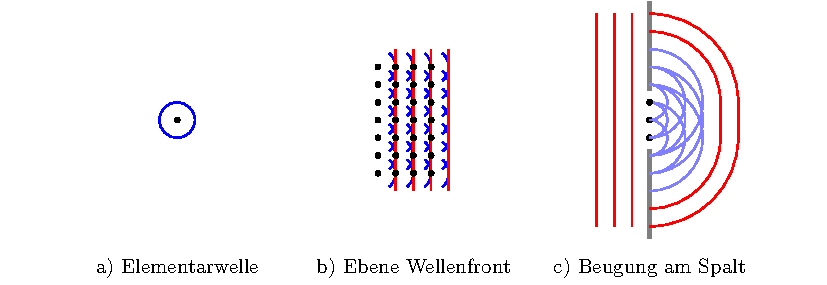
\includegraphics[width=120mm]{papers/opt/images/huygens.pdf}
    \caption{Gemäss dem Prinzip von Huygens kann eine Welle als Summe unendlicher Elementarwellen aufgefasst werden.
    Wenn diese Welle auf ein Hindernis trifft, entsteht dahinter eine neue, gebogene Wellenfront.}
    \label{opt:fig:huygens}
\end{figure}

\subsection{Grundlagen Wellentheorie}
\label{opt:subsection:huygens}
Das Prinzip der optischen Fouriertransformation basiert auf der Beugung von Wellen.
Im folgenden wird die Beugung grob abgehandelt, für eine weitere Behandlung wird auf Kapitel 32 aus dem Physikbuch der HSR \cite{opt:HSR:Physik2} verwiesen.

Qualitativ lässt sich die Beugung mit dem Prinzip von Huygens erklären. 
Abbildung \ref{opt:fig:huygens} zeigt den konzeptionellen Aufbau einer Welle.
Diese lässt sich als Superposition von unendlichen Elementarwellen betrachten.
An jedem Punkt der so entstehenden Wellenfront entsteht eine neue Elementarwelle und daraus wieder eine neue Wellenfront.
Wenn jetzt ein Hindernis die Fortpflanzung der Welle stoppt, bildet sich aus den nicht abgeblockten Elementarwellen eine neue Wellenfront.
Diese ist jetzt jedoch nicht mehr eben, da die generierenden Elementarwellen auf ein endliches Intervall beschränkt sind.

Dieses Phänomen lässt sich beispielsweise auch am Strand beobachten. 
Wenn eine Welle durch eine Öffnung hindurch kommt, breitet sie sich dahinter kreisförmig wieder aus.

\begin{figure}
    \centering
    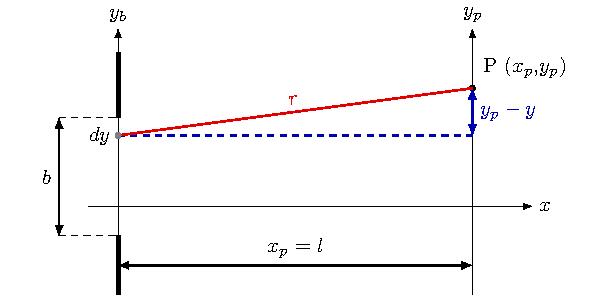
\includegraphics[width=90mm]{papers/opt/images/derivation.pdf}
    \caption{Beugung am Spalt: Die ebene Welle kommt von links her an den Spalt. 
    Von allen $dy$ geht eine Elementarwelle gemäss Kapitel \ref{opt:subsection:huygens} aus, welche sich am Auswertepunkt $P$ aufsummiert.}
    \label{opt:fig:geometricalShape}
\end{figure}

\subsection{Herleitung Beugungsintegrale}
In dieser Herleitung wird darauf eingegangen, wie aus dem allgemein gültigen Beugungsintegral durch die Fressnel-Approximation das gleichnamige Beugungsintegral und durch die Fraunhofer-Approximation das Fraunhofer-Beugungsintegral hergeleitet werden kann.

Betrachten wir zuerst, wie in TODO gezeigt, eine unendlich dünne linienförmige Lichtquelle, welche sich axial in beide Richtungen unendlich weit erstreckt.
Verallgemeinert kann es sich bei dieser Art von Quelle um eine beliebige elektromagentische Quelle handeln.
Somit kann durch Anwenden der ersten Maxwellschen Gleichung
\begin{equation}
\oint_{S=\partial V} \varepsilon\vec{E} \cdot\, d\vec{S}
=
\int_{V}\rho\, dV
\end{equation}
die elektrische Feldstärke $\vec{E}$ an jedem beliebigen Punkt in Abhängigkeit des radialen Abstandes $r$ berechnet werden.
Dabei ist $\varepsilon$ die dielektrische Feldkonstante, $\varrho$ die Ladungsdichte und $V$ das Volumen über dessen Oberfläche $S$ integriert werden muss.
Angewendet auf die gegebene Geometrie des Zylindermantels lässt sich diese Gleichung mittels $dS = r d\varphi dl$ als
\begin{align}
\int_{0}^{a}\int_{0}^{2\pi} \varepsilon E\cdot 1 \cdot r\, d\varphi dl
&=
Q
\\
2\pi ra\varepsilon E
&=
Q
\end{align}
schreiben.
Die Deckflächen können aufgrund der infiniten Länge des Zylinders vernachlässigt werden.
$Q$ beschreibt die durch den Zylindermantel eingeschlossene Ladung und $a$ dessen Länge.
Zu beachten sei zudem, dass die normierten vektoriellen Grössen $\hat{E}$ und $\hat{S}$ parallel verlaufen und sich ihr Skalarprodukt dementsprechend zu 1 vereinfacht.
Nach der elektrischen Feldstärke umgeformt lautet die Gleichung
\begin{equation}
E(r)
=
\frac{Q}{2\pi\varepsilon a} \cdot \frac{1}{r}
=
C \cdot \frac{1}{r}
,
\label{opt:equation:E}
\end{equation}
wobei der konstante Anteil als $C$ zusammengefasst wurde.

Angenommen eine planare elektromagentische Welle, siehe TODO, treffe nun auf eine Blende mit einer unendlich langen und $b$ breiten Öffnung.
Ganz allgemein lässt sich jede Welle als
\begin{equation}
\zeta(x, t)
=
\zeta_0 \cdot e^{j(\omega t - \vec{k}\cdot\vec{x})}
\label{opt:equation:wave}
\end{equation}
ausdrücken.
Wie in Kapitel \ref{opt:subsection:huygens} gezeigt, wird diese Welle an der Blende gebogen.
In Abhängigkeit von $b$ breitet sich die Welle anschliessend annähernd kreisförmig als neue Wellenfront weiter.
Dieses Verhalten der kreisförmigen Ausbreitung kann mittels der zuvor betrachteten Linienquellen modelliert werden.
Infinit viele dieser Linienquellen seien nun nebeneinander entlang der Öffnungsbreite $b$ angereiht.
Die Auswirkung dieser Quellen kann nun an jedem beliebigen Punkt hinter der Blende durch Superposition der einzelnen Quelleneinflüsse berechnet werden.

Ein Schirm werde nun im Abstand $l$ hinter der Blende angebracht, an welchem die elektrische Feldstärke auf verschiedenen Höhen $y_p$ gemessen werden soll.
Aus der geometrischen Anordnung in Abbildung \ref{opt:fig:geometricalShape} geht hervor, dass
\begin{equation}
r
=
\sqrt{l^2 + (y_p-y)^2}
=
l \sqrt{1 + \frac{(y_p-y)^2}{l^2}}
\label{opt:equation:distance_r}
\end{equation}
beträgt. All diese kleinen Einflüsse $dE$ der Linienquellen mit Breite $dy$ superponieren sich, wie bereits erwähnt, zur gesamten elektrischen Feldstärke am Auswertungspunkt.
Ein solcher Einfluss lässt sich nun mittels der Gleichungen~\ref{opt:equation:E} und \ref{opt:equation:wave} als
\begin{equation}
dE
=
E(r) \cdot \zeta(r, t) \cdot dy
=
\frac{C}{r} \cdot \zeta_0 \cdot e^{j(\omega t - \vec{k}\cdot\vec{r})} \cdot dy
\end{equation}
beschreiben.
Werden die Einflüsse der Linienquellen über den Spalt integriert, ergibt sich
\begin{equation}
E(y_p, t)
=
\int_{y_b}^{y_b+b}\frac{C\zeta_0}{r} \cdot e^{j(\omega t - \vec{k}\cdot\vec{r})} \,dy
=
C\zeta_0 \cdot \int_{y_b}^{y_b+b}\frac{e^{j(\omega t - \vec{k}\cdot\vec{r})}}{r} \,dy
.
\end{equation}

Soll nun aber anstelle eines einzelnen Spalts mehrere davon in beliebigen Abständen zueinander betrachtet werden, kann dieses Integral mit Hilfe der Blendenfunktion
\begin{equation}
f(y)
\in
(0, 1)
\end{equation}
dargestellt werden.
Zu beachten ist, dass $f(y)$ nicht nur die Werte 0 und 1, sondern auch jegliche Werte dazwischen annehmen kann.
Dies würde einer teilweise transparenten Blende entsprechen.
Somit folgt als allgemeinste Form
\begin{align}
E(y_p, t)
=
C\zeta_0 \cdot \int_{-\infty}^{\infty}f(y)\cdot\frac{e^{j(\omega t - \vec{k}\cdot\vec{r})}}{r} \,dy
.
\label{opt:equation:integral_general}
\end{align}
Dieses Integral ist für jeden Auswertungspunkt allgemein gültig.
Wie sich aber zeigen wird, ist dieses Integral, genauer gesagt $r$ aus Gleichung~\ref{opt:equation:distance_r}, nicht fundamental genug, um es analytisch lösen zu können.
Die folgenden Approximationen von $r$ sollen dabei diese Hürde umgehen.

\subsubsection{Fressnel-Approximation}
In näherer Umgebung um die Blende wird hierfür die Fressnel-Approximation angewendet.
Für weitere Schritte soll die Bedingung
\begin{equation}
y, y_p
\ll
l
\label{opt:equation:condition_fressnel}
\end{equation}
gelten.
Durch Anwenden der Binominalexpansion
\begin{equation}
(1 + \varepsilon)^n
\approx
1 + n\varepsilon
,
\end{equation}
unter der Voraussetzung, dass $\varepsilon \ll 1$ gilt, ist es möglich den Wurzelausdruck aus Gleichung~\ref{opt:equation:distance_r} noch weiter zu vereinfachen.
Mit Hilfe der Vorbedingungen aus Gleichung~\ref{opt:equation:condition_fressnel} ist
\begin{equation}
(y_p-y)^2
\ll
l^2
\end{equation}
gegeben.
Somit kann die Bedingung für
\begin{equation}
\varepsilon
=
\frac{(y_p-y)^2}{l^2}
\ll
1
\label{opt:equation:condition_epsilon}
\end{equation}
eingehalten werden.
Gleichung~\ref{opt:equation:distance_r} vereinfacht sich demnach näherungsweise zu
\begin{equation}
r
=
l \sqrt{1 + \frac{(y_p-y)^2}{l^2}}
\approx
l \left(1 - \frac{(y_p-y)^2}{2l^2}\right)
=
l - \frac{(y_p-y)^2}{2l}
.
\label{opt:equation:distance_r_fressnel}
\end{equation}
Durch Ausklammern von Konstanten und Einsetzen der Gleichung~\ref{opt:equation:distance_r_fressnel} vereinfacht sich das Integral aus Gleichung~\ref{opt:equation:integral_general} weiter zu
\begin{align}
E(y_p, t)
&=
C\zeta_0 \cdot e^{j\omega t} \cdot \int_{-\infty}^{\infty}f(y)\cdot\frac{e^{-j\vec{k}\cdot\vec{r}}}{r} \,dy
\\
&=
C\zeta_0 \cdot e^{j\omega t} \cdot \int_{-\infty}^{\infty}f(y)\cdot\frac{e^{-jkr \cdot 1}}{r} \,dy
\\
&=
C\zeta_0 \cdot e^{j\omega t} \cdot \int_{-\infty}^{\infty}f(y)\cdot\frac{e^{-jkl} \cdot e^{jk\frac{(y_p-y)^2}{2l}}}{l - \frac{(y_p-y)^2}{2l}} \,dy
\\
&=
C\zeta_0 \cdot e^{j\omega t} \cdot e^{-jkl} \cdot \int_{-\infty}^{\infty}f(y)\cdot\frac{e^{jk\frac{(y_p-y)^2}{2l}}}{l - \frac{(y_p-y)^2}{2l}} \,dy
.
\end{align}
Wiederum konnte das Skalarprodukt der normierten Grössen $\hat{k}$ und $\hat{r}$ aufgrund Parallelität als 1 gekürzt geschrieben werden.
Des Weiteren kann der Ausdruck $l - \frac{(y_p-y)^2}{2l}$ im Nenner des Integrals als $l$ vereinfacht werden.
Zulässig ist dies nur, weil $(y_p - y)^2 \ll l$ erfüllt ist.
Dasselbe Prinzip darf jedoch nicht auf den Exponenten angewandt werden, da dieser mit dem Faktor der Wellenzahl multipliziert wird und der Term $k \frac{(y_p-y)^2}{2l}$ somit nicht vernachlässigbar klein wird.
Der Zeitpunkt der Auswertung sei nicht von Interesse, da dieser lediglich den Momentanwert der Welle beeinflusst.
Mittels $t = 0$ ergibt sich daraus
\begin{align}
E(y_p, t = 0)
&=
C\zeta_0 \cdot e^{j\omega t} \cdot e^{-jkl} \cdot \int_{-\infty}^{\infty}f(y)\cdot\frac{e^{jk\frac{(y_p-y)^2}{2l}}}{l} \,dy
\\
&=
\frac{C\zeta_0}{l} \cdot 1 \cdot e^{-jkl} \cdot \int_{-\infty}^{\infty}f(y)\cdot e^{jk\frac{(y_p-y)^2}{2l}} \,dy
\\
&=
\frac{C\zeta_0}{l} \cdot e^{-jkl} \cdot \int_{-\infty}^{\infty}f(y)\cdot e^{jk\frac{(y_p^2 - 2y_py + y^2)}{2l}} \,dy
.
\label{opt:equation:integral_fressnel}
\end{align}
Das hiermit erhaltene Integral wird auch als das Fressnel Beugungsintegral bezeichnet und ist in näherer Umgebung um die Blende gültig.

\subsubsection{Fraunhofer-Approximation}
Wird die Distanz zwischen Blende und Auswertungspunkt noch weiter erhöht, ist es möglich, mit der Fraunhofer-Approximation eine noch einfachere Form des Beugungsintegrals zu erhalten.
Sei nun
\begin{equation}
y
\ll
y_p
\ll
l
\end{equation}
gegeben, kann der Ausdruck $y_p^2 - 2y_py + y^2$ aus Gleichung~\ref{opt:equation:integral_fressnel} weiter approximiert werden.
Unter Berücksichtigung dieser Bedingung sei $y^2 \ll 2y_py$, wodurch der Term $y^2$ vernachlässigt werden kann.
Daraus folgt
\begin{align}
E(y_p)
&=
\frac{C\zeta_0}{l} \cdot e^{-jkl} \cdot \int_{-\infty}^{\infty}f(y)\cdot e^{jk\frac{(y_p^2 - 2y_py)}{2l}} \,dy
\\
&=
\frac{C\zeta_0}{l} \cdot e^{-jkl} \cdot e^{jk\frac{y_p^2}{2l}} \cdot \int_{-\infty}^{\infty}f(y)\cdot e^{-jk\frac{y_py}{l}} \,dy
\\
&=
\frac{C\zeta_0}{l} \cdot e^{-jk\left(l-\frac{y_p^2}{2l}\right)} \cdot \int_{-\infty}^{\infty}f(y)\cdot e^{-j\frac{ky_p}{l}y} \,dy
.
\label{opt:equation:integral_fraunhofer}
\end{align}

\subsubsection{Intensität}
Diese elektrische Feldstärke kann leider nicht direkt auf dem Schirm beobachtet werden.
Denn ein Beobachter, sei es das menschliche Auge oder ein Kamera Chip, kann negative und positive Amplituden sowie komplexwertige Grössen nicht unterscheiden.
Gesehen werden kann lediglich die Intensität $I$, welche sich proportional zur elektrischen Feldstärke verhält.
Auf Konstanten wird vorerst verzichtet, woraus sich aus Gleichung~\ref{opt:equation:integral_fraunhofer}
\begin{align}
I(y_p)
&\propto
|E(y_p)|^2
\\
&=
\left(\frac{C\zeta_0}{l} \cdot \int_{-\infty}^{\infty}f(y)\cdot e^{-j\frac{ky_p}{l}y} \,dy\right)^2
\\
&=
\frac{C^2\zeta_0^2}{l^2}\cdot \left(\int_{-\infty}^{\infty}f(y)\cdot e^{-j\frac{ky_p}{l}y} \,dy\right)^2
\end{align}
ergibt.

\subsubsection{Vergleich mit der Fouriertransformation}

